\section{Introduzione}
\subsection{Dati di progetto}
Lo studio e la progettazione della trasmissione in esame parte da alcune linee guida fornite dall'azienda COMER INDUSTRIES. \\
Il riduttore è dotato di un ingresso a 312RPM e 2 uscite (Output 1 e 2, coassiali) secondo le velocità indicate in Fig.\ref{fig:Ingombri}. Nello stesso schema sono quindi riportati gli interassi da mantenere, gli ingombri massimi della cassa, e i sensi di rotazione. Gli scostamenti ammessi sulle velocità di uscita sono di ±1.5\%.\\
\begin{figure}[h]
    \centering
    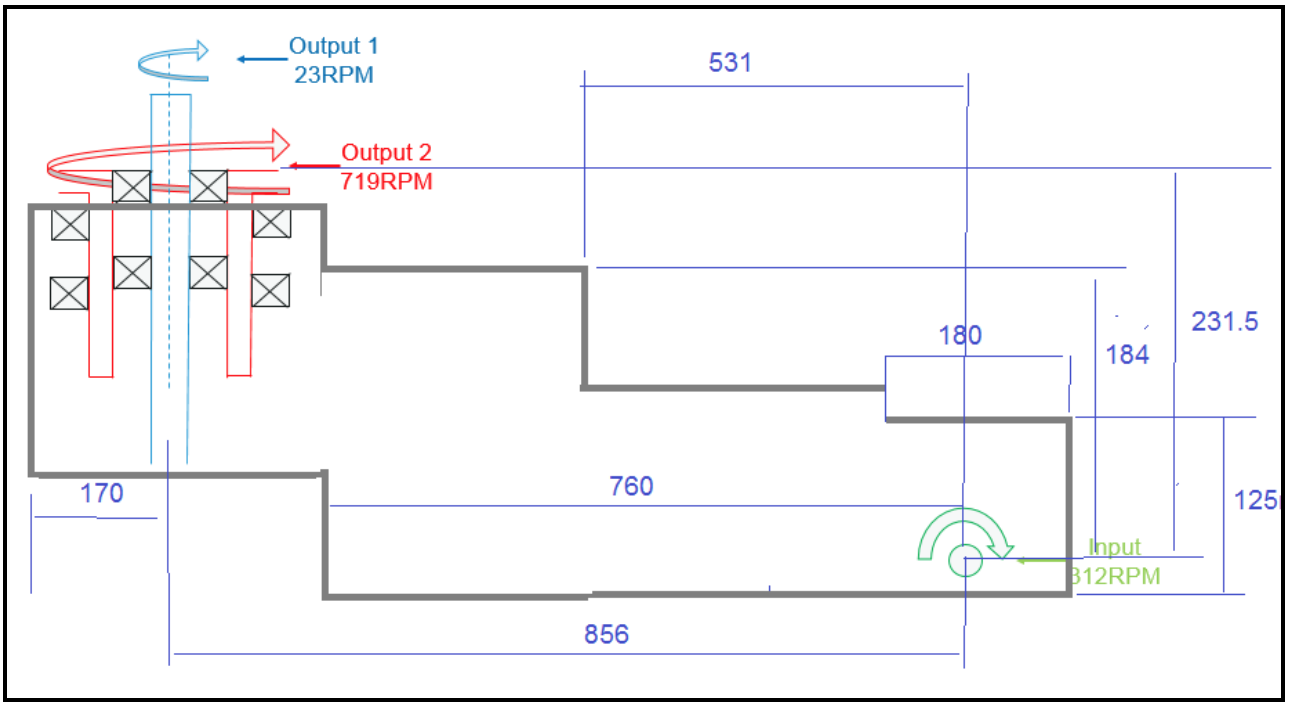
\includegraphics[scale=0.5]{Immagini/Ingombri.png}
    \caption{Ingombri di massima e velocità di rotazione}
    \label{fig:Ingombri}
\end{figure}

Con questi dati, dopo vari tentativi, sono state scelte le dimensioni di massima che rientrassero negli ingombri sopra citati e si è ottenuta la seguente configurazione. Sono state inoltre nominati gli accoppiamenti tra le ruote per avere una maggiore chiarezza nello svolgimento. 
\begin{figure}[h]
    \centering
    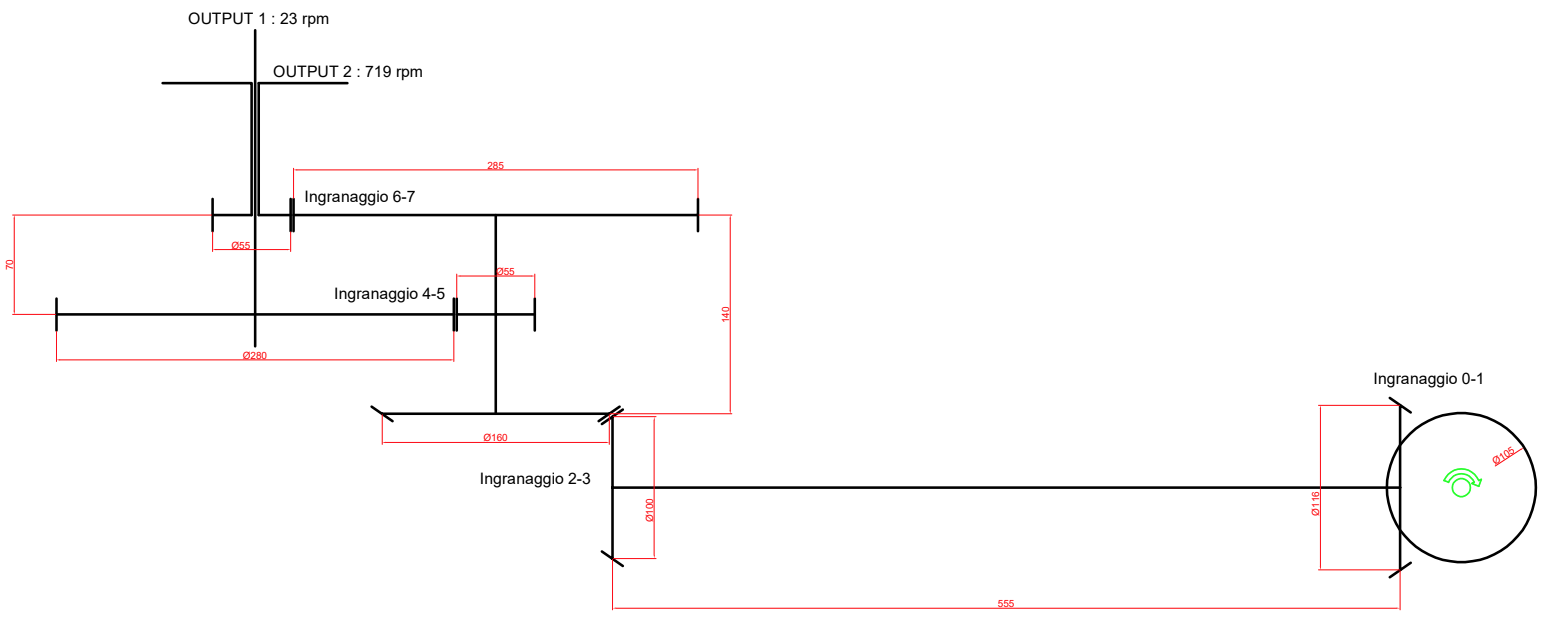
\includegraphics[scale=0.6]{Immagini/DenominazioneRiduttore.png}
    \caption{Approccio al dimensionamento e denominazione degli accoppiamenti tra le ruote}
    \label{fig:DenominazioniRuote}
\end{figure}
